
%! Author = UserHome
%! Date = 02.12.2024

\chapter{Heuristické algoritmy}

Táto kapitola sa zameriava na algoritmy, ktoré využívajú heuristické metódy na hľadanie riešení. Tieto algoritmy sú navrhnuté tak, aby rýchlo našli riešenie, aj keď nemusia zaručiť nájdenie optimálneho výsledku. Príkladmi sú algoritmy ako min-max konflikt a hill climbing, ktoré sa opierajú o lokálne úpravy aktuálneho stavu šachovnice.

\section*{Min-max konflikt}
Najprv sa dámy umiestnia na šachovnicu do náhodných pozícií z domény ako je znázornené na obrázku \ref{fig:min-max-zero-step}. Tento krok sa začína náhodným výberom kráľovnej s aspoň 1 konfliktom. Potom sa presunie na pozíciu v doméne, kde má najmenej konfliktov. Tento krok je znázornený na obrázku \ref{fig:min-max-step}. Tieto kroky sa vykonávajú, kým sa nenájde riešenie alebo kým sa nevyčerpá limit krokov.
\begin{figure}
    \centering
    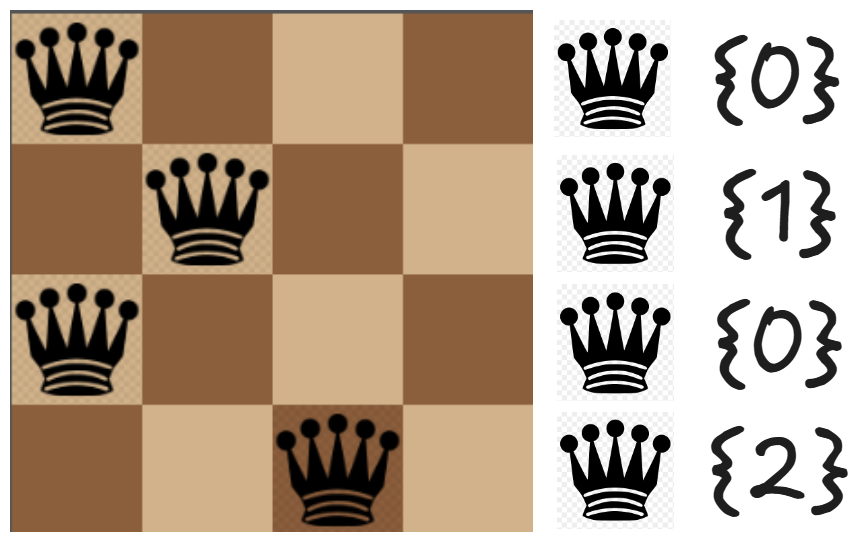
\includegraphics[width=0.6\textwidth]{figs/min-max/min-max-zero-step}
    \caption{Počiatočný stav pri min-max konflikte}
    \label{fig:min-max-zero-step}
\end{figure}
\begin{figure}
    \centering
    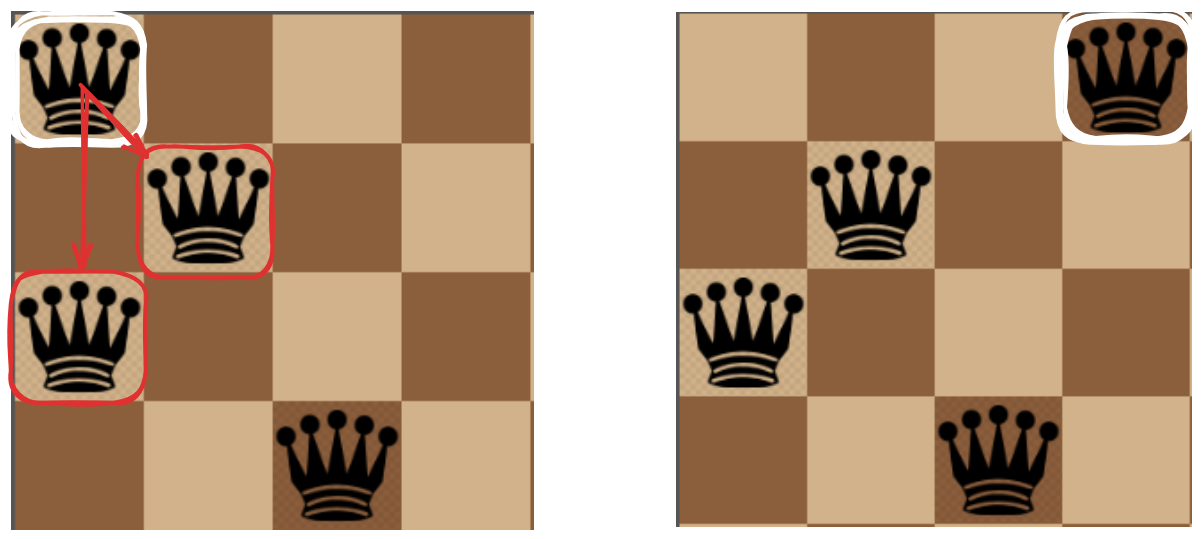
\includegraphics[width=0.8\textwidth]{figs/min-max/min-max-step}
    \caption{Presun dámy na pozíciu s najmenším počtom konfliktov pri min-max konflikte}
    \label{fig:min-max-step}
\end{figure}

\section*{HillClimbing}
